\section{El men� del juego}
El men� del juego viene representado en la figura~\ref{s7:fig:menu}. Los
botones est�n creados de igual manera que las acciones vistas en las
secciones anteriores. Asociado a cada bot�n hay un script encargado de
cargar el men� correspondiente y colorear el fondo de acuerdo a si se ha
superado o no. Para realizar la carga de niveles y almacenar los niveles
superados se utiliza una clase est�tica.
\begin{figure}
  \centering
  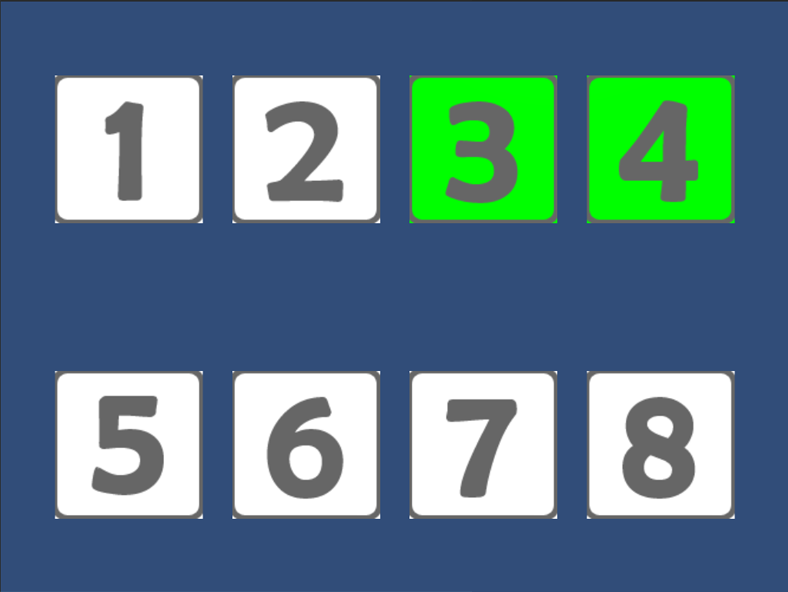
\includegraphics[width=0.7\textwidth]{images/interfaz_menu.png}
  \caption{Escena con el men�}
  \label{s7:fig:menu}
\end{figure}


\begin{lstlisting}[caption={Menu.cs}]
using UnityEngine;
using System.Collections;

/**
 * Clase estatica que almacena el estado actual de los niveles, asi como del nivel actual
 **/
public static class levelLoad{
  public static int level = -1;
  public static bool[] levelPassed = {false, false, false, false,
    false, false, false, false};
}


/**
 * Listener de los botones del menu. Carga el menu correspondiente
 **/
public class Menu : MonoBehaviour {

  public int level;
  public Material bck_green;
  

  //Comprobamos si el nivel se ha superado y lo pintamos de verde
  public void Start(){
    //cambiar el material del fondo
    if(levelLoad.levelPassed[this.level-1]){
      MeshRenderer rmat;
      rmat = this.transform.parent.GetComponentInChildren<MeshRenderer>();
      
      rmat.material = this.bck_green;	
    }
  }
  

  public void OnMouseUpAsButton(){
    if(this.level==0){ //cargamos el menu
      Application.LoadLevel("_Scene_menu");
    }
    else {//caso contrario cargamos el nivel correspondiente
      levelLoad.level = this.level;
      
      Application.LoadLevel("_Scene_0");
    }
  }
}
\end{lstlisting}
